\documentclass[aspectratio=169]{beamer}
\usetheme{CambridgeUS}
\usepackage{array}

\title[Two-Stage Folded-Cascode Op-Amp]{A Two-Stage Folded-Cascode Op-Amp in 180\,nm CMOS}
\author{Haoyu Li}
\date{November 16, 2026}

\begin{document}

\begin{frame}
  \titlepage
\end{frame}

\begin{frame}{First-Pass Amplifier Core and Bias Network}
  \centering
  \makebox[\linewidth][c]{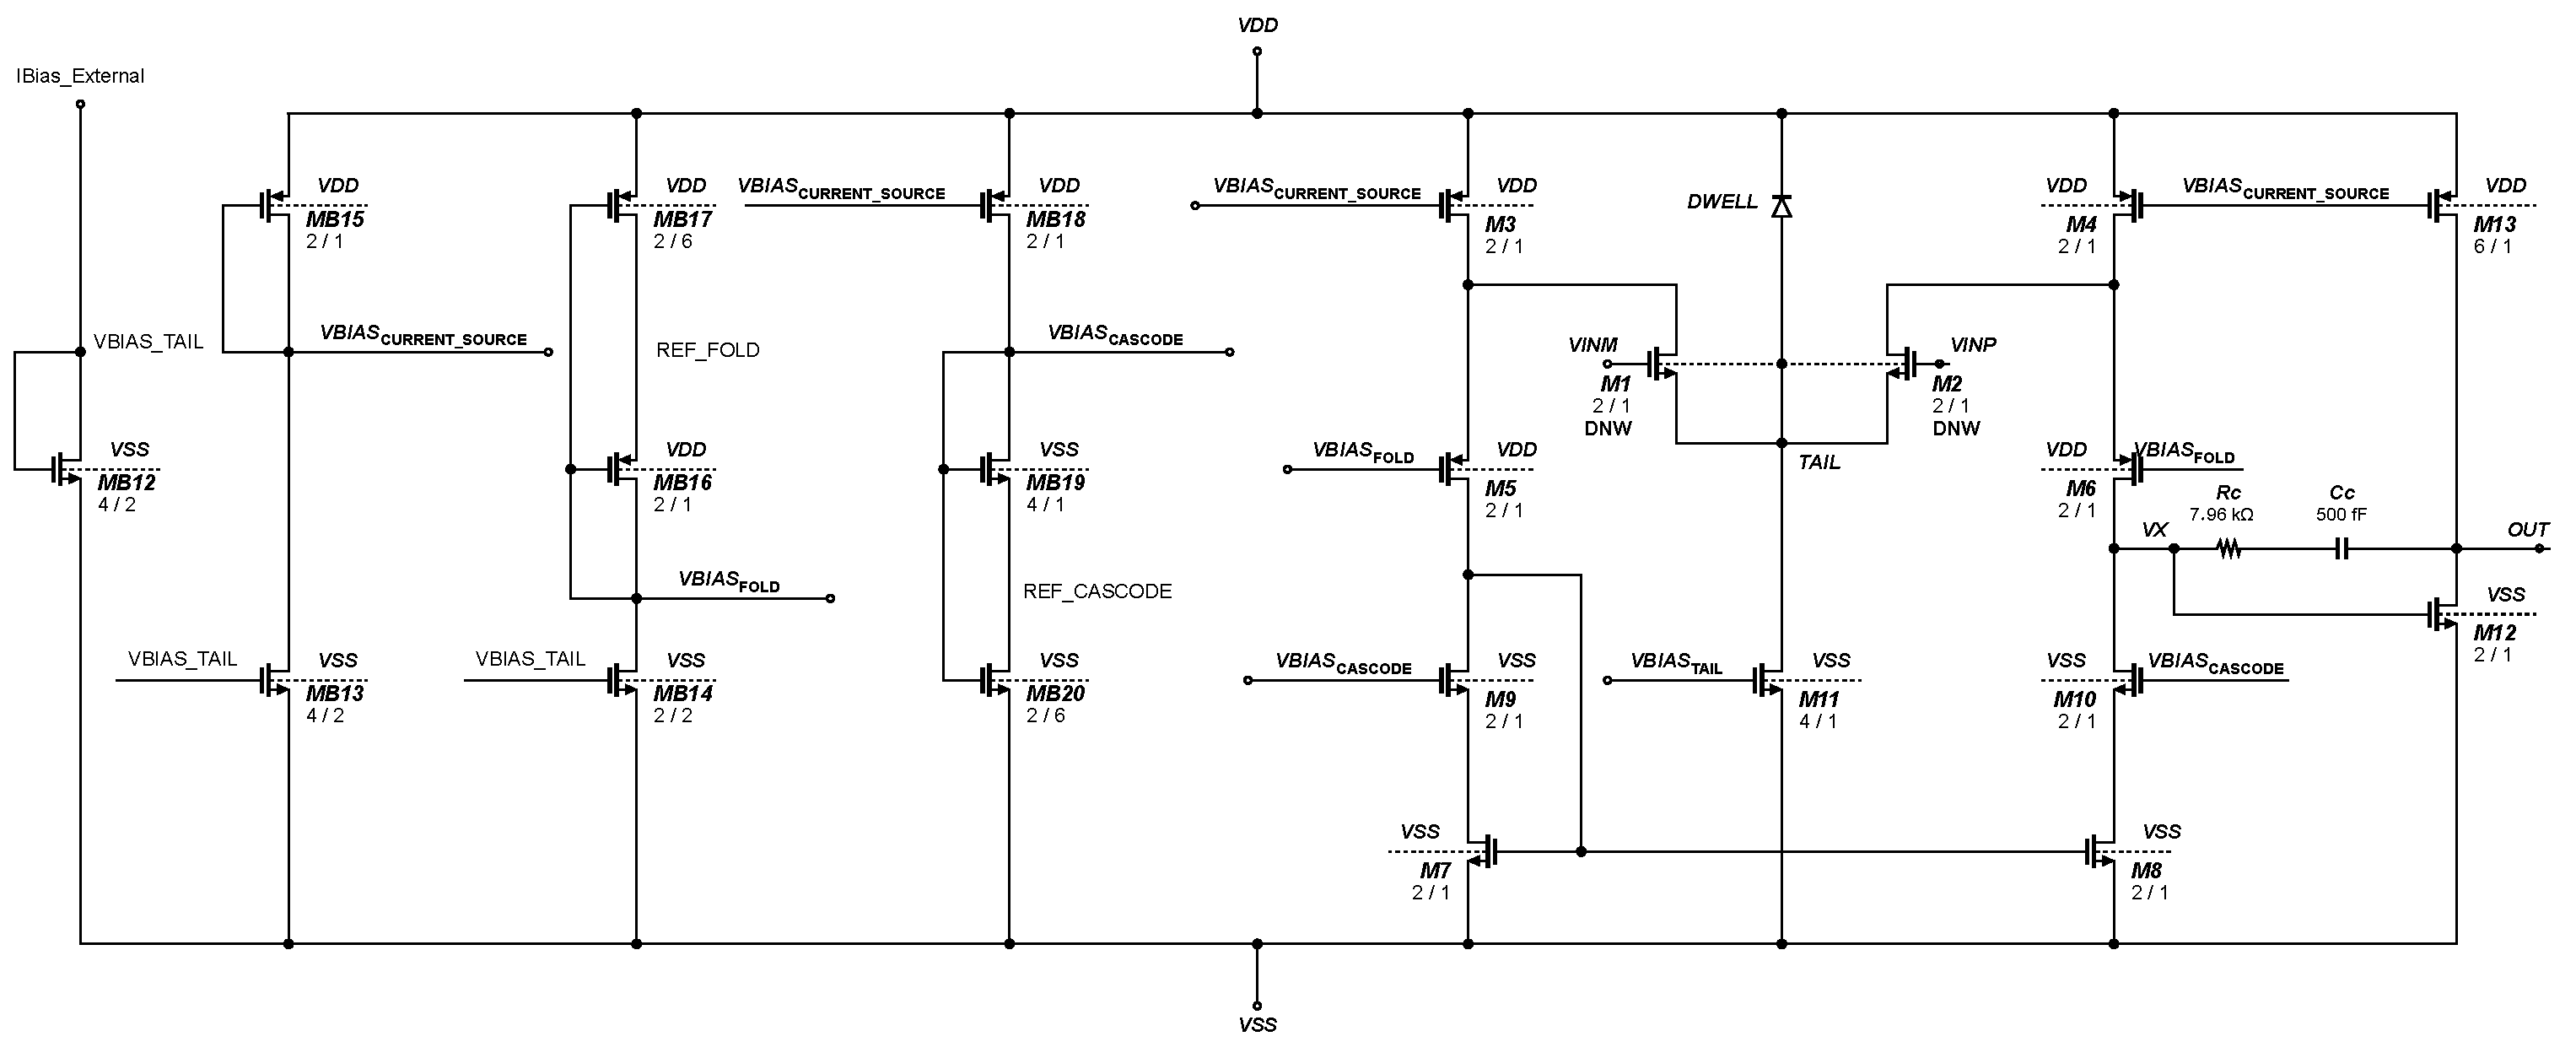
\includegraphics[width=.97\paperwidth]{images/first-pass-core-and-bias.pdf}}
\end{frame}

\begin{frame}{First-Pass Amplifier Core Sizing}
  \footnotesize
  \[
    I_{11}^{*}=C_c\max(S_\uparrow,S_\downarrow)=10\,\mu\mathrm A,\quad
    I_{13}^{*}=(C_L+C_c)S_\uparrow=30\,\mu\mathrm A,\quad
    I_{1,2}^{*}=I_{\rm fold}^{*}=I_{11}^{*}/2=5\,\mu\mathrm A
  \]
  \vspace{-.8em}
  \[
    G_{m1}^{*}=2\pi f_u C_c=62.8\,\mu\mathrm S,\quad
    g_{m12}^{*}=2\pi f_u C_L\tan(\mathrm{PM})=125.7\,\mu\mathrm S,\quad
    R_c=1/g_{m12}^{*}=7.96\,\mathrm{k}\Omega
  \]
  \vspace{-.4em}
  \renewcommand{\arraystretch}{1.2}
  \begin{tabular*}{\linewidth}{@{\extracolsep{\fill}}llr@{}}
    \textbf{MOS} & \textbf{Selection from saturated device sweeps} & \textbf{\(W/L\) (\(\mu\)m)}\\
    \hline
    M12 & \(I_{12}\simeq I_{13}^{*},\quad g_{m12}\ge g_{m12}^{*}\) & \(2/1\)\\
    M3, M4; M13 & \(V_{SG3}=V_{SG13},\quad I_3\ge I_1^{*}+I_{\rm fold}^{*},\quad
      g_{m12}(r_{o12}\parallel r_{o13})\ge10^{23/20}\) & \(2/1;\ 6/1\)\\
    M1, M2 & \(G_{m1}^{*}/I_1^{*}\to J_D,\quad W_0=I_1^*/J_D,\quad I_1\ge I_1^*,\quad g_{m1}\ge G_{m1}^{*}\) & \(2/1\)\\
    M11 & \(V_{DS11}=V_{\rm CM}-V_{GS1},\quad V_{GS11}=V_{GS,\rm MB12},\quad I_{11}\ge I_{11}^{*}\) & \(4/1\)\\
    M5--M10 & \(L=\min\{\ell\in\{1,2\}\,\mu\mathrm m:\ G_{m1}^{*}(R_\uparrow\parallel R_\downarrow)\ge10^{40/20}\}\) & \(2/1\)\\
  \end{tabular*}
  \smallskip
  \[
    R_\uparrow\simeq g_{m6}r_{o6}(r_{o2}\parallel r_{o4}),\qquad
    R_\downarrow\simeq g_{m10}r_{o10}r_{o8}.
  \]
  \centering \(^{*}\) design target\qquad \(J_D=I_D/W\)\qquad \(W\in\{2,4,6,\ldots\}\,\mu\mathrm m\)
\end{frame}

\begin{frame}{First-Pass Bias Network Sizing}
  \centering\small
  \[
    I_{\rm ref}=10\,\mu\mathrm A,\qquad I_{3,4}^{*}=10\,\mu\mathrm A,\qquad
    I_{\rm fold}^{*}=5\,\mu\mathrm A
  \]
  \renewcommand{\arraystretch}{1.14}
  \begin{tabular*}{\dimexpr\linewidth-3pt\relax}{@{\extracolsep{\fill}}llr@{}}
    \textbf{Device} & \textbf{Sizing relation} & \textbf{\(W/L\) (\(\mu\)m)}\\
    \hline
    MB12 & \(I_{\rm MB12}=I_{\rm ref}\) (reference geometry given) & \(4/2\)\\
    MB13 & \(W=W_{\rm MB12}\,I_3^{*}/I_{\rm ref},\quad L=L_{\rm MB12}\) & \(4/2\)\\
    MB14 & \(W=W_{\rm MB12}\,I_{\rm fold}^{*}/I_{\rm ref},\quad L=L_{\rm MB12}\) & \(2/2\)\\
    MB15 & \((W,L)_{\rm MB15}=(W,L)_3\) & \(2/1\)\\
    MB16 & \((W,L)_{\rm MB16}=(W,L)_5\) & \(2/1\)\\
    MB18 & \(W=W_{\rm MB15}\,I_{\rm ref}/I_3^{*},\quad L=L_{\rm MB15}\) & \(2/1\)\\
    MB19 & \(W=W_9\,I_{\rm ref}/I_{\rm fold}^{*},\quad L=L_9\) & \(4/1\)\\
    MB17, MB20 & DC trial sizes for triode operation & \(2/6\) each
  \end{tabular*}
\end{frame}

\begin{frame}{Open-Loop and Unity-Gain Testbench}
  \centering
  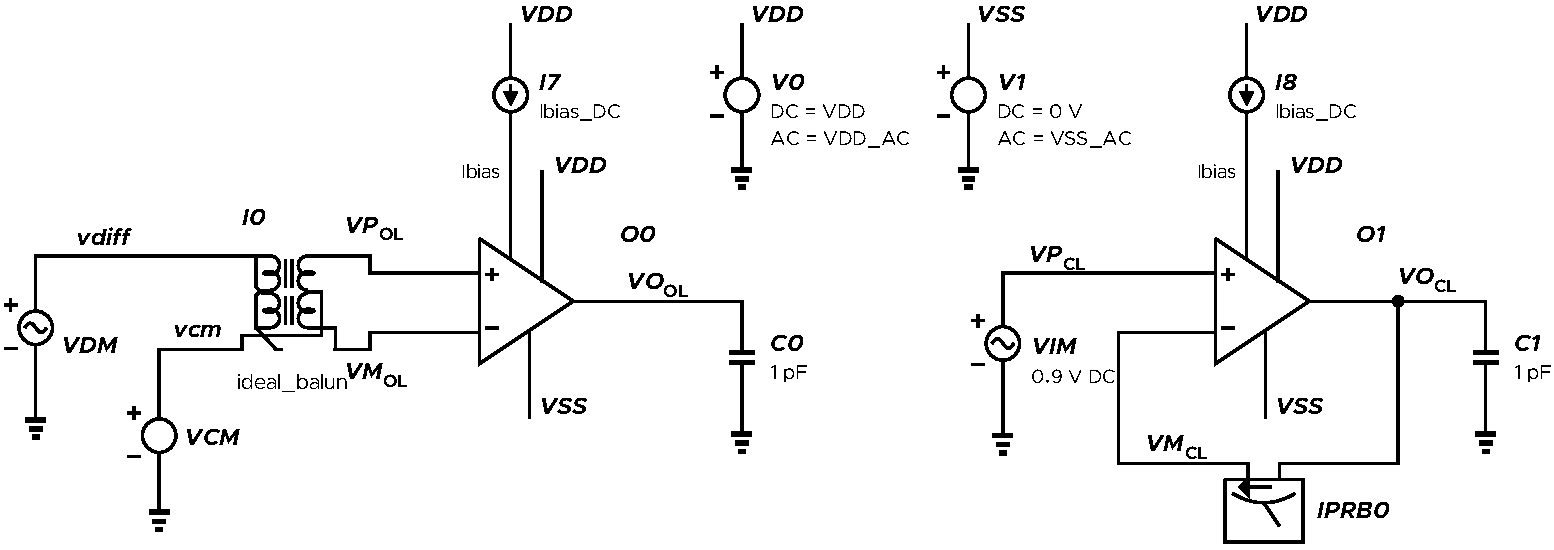
\includegraphics[width=\linewidth,height=0.78\paperheight,keepaspectratio]{images/testbench.pdf}
\end{frame}

\DeclareFontFamily{TU}{adecode}{}
\DeclareFontShape{TU}{adecode}{m}{n}{<->"[lmmono10-regular.otf]"}{}
\newcommand{\ade}[1]{{\fontfamily{adecode}\selectfont\detokenize{#1}}}
\newcommand{\adetestrow}[1]{\multicolumn{2}{@{}l}{\color{darkred}\ade{#1}}\tabularnewline}
\newenvironment{adeoutputs}{%
  \fontsize{7.5}{8.2}\selectfont
  \renewcommand{\arraystretch}{.91}
  \begin{tabular}{@{}>{\raggedright\arraybackslash}p{.225\linewidth}@{\hspace{.012\linewidth}}>{\raggedright\arraybackslash}p{.759\linewidth}@{}}
    \textbf{Test / output name} & \textbf{ADE Calculator expression} \\[.2em]
    \hline
    \noalign{\vskip .25em}
}{\end{tabular}}

\begingroup
\setbeamertemplate{navigation symbols}{}
\begin{frame}{Simulation Setup --- DC and Differential Gain}
  \begin{adeoutputs}
    \adetestrow{DC_bias}
    \ade{Vout_CL} & \ade{VDC("/VO_CL")} \\[.16em]
    \adetestrow{test_OL_DM_offset}
    \ade{VDM_OFFSET} & \ade{cross(VS("/VO_OL") (VAR("VDD") / 2) 1 "either" nil nil)} \\[.16em]
    \adetestrow{test_OL_ICMR}
    \ade{ICMR_Lower} & \ade{if((value(calcVal("ICMR_region_error" "test_OL_ICMR") 0) < 0.5) then 0 else}\newline
      \hspace*{.55em}\ade{cross(calcVal("ICMR_region_error" "test_OL_ICMR") 0.5 1 "falling" nil nil))} \\[.02em]
    \ade{ICMR_Upper} & \ade{if((value(calcVal("ICMR_region_error" "test_OL_ICMR") VAR("VDD")) < 0.5) then}\newline
      \hspace*{.55em}\ade{VAR("VDD") else cross(calcVal("ICMR_region_error" "test_OL_ICMR") 0.5 1}\newline
      \hspace*{.55em}\ade{"rising" nil nil))} \\[.16em]
    \adetestrow{test_OL_power_DC}
    \ade{PowerDC_vs_VCM} & \ade{(VAR("VDD") * (IS("/O0/VDD") + IS("/I7/PLUS")))} \\[.02em]
    \ade{PowerDC_nominal} & \ade{value(calcVal("PowerDC_vs_VCM" "test_OL_power_DC") VAR("VCM_DC"))} \\[.02em]
    \ade{PowerDC_MAX_ICMR} & \ade{ymax(clip(calcVal("PowerDC_vs_VCM" "test_OL_power_DC") calcVal("ICMR_Lower"}\newline
      \hspace*{.55em}\ade{"test_OL_ICMR") calcVal("ICMR_Upper" "test_OL_ICMR")))} \\[.16em]
    \adetestrow{test_OL_diff_AC}
    \ade{A0_dB_1Hz} & \ade{value(dB20((VF("/VO_OL") / (VF("/VP_OL") - VF("/VM_OL")))) 1)} \\[.02em]
    \ade{fp1} & \ade{cross(calcVal("Aol_dB") (calcVal("A0_dB_1Hz") - 3) 1 "falling" nil nil)} \\[.02em]
    \ade{GBW} & \ade{gainBwProd((VF("/VO_OL") / (VF("/VP_OL") - VF("/VM_OL"))))} \\[.02em]
    \ade{UGF} & \ade{unityGainFreq((VF("/VO_OL") / (VF("/VP_OL") - VF("/VM_OL"))))} \\[.02em]
    \ade{Phase Margin} & \ade{phaseMargin((VF("/VO_OL") / (VF("/VP_OL") - VF("/VM_OL"))))} \\[.16em]
  \end{adeoutputs}
\end{frame}

\begin{frame}{Simulation Setup --- Rejection and Large-Signal Tests}
  \begin{adeoutputs}
    \adetestrow{test_OL_comm_AC}
    \ade{CMRR_dB} & \ade{(calcVal("Aol_dB" "test_OL_diff_AC") - calcVal("Acm_dB" "test_OL_comm_AC"))} \\[.02em]
    \ade{CMRR_max_dB} & \ade{ymax(calcVal("CMRR_dB" "test_OL_comm_AC"))} \\[.16em]
    \adetestrow{test_OL_PSRRp_AC}
    \ade{PSRRp_dB} & \ade{(calcVal("Aol_dB" "test_OL_diff_AC") - calcVal("Avdd_dB" "test_OL_PSRRp_AC"))} \\[.02em]
    \ade{PSRRp_max_dB} & \ade{ymax(calcVal("PSRRp_dB" "test_OL_PSRRp_AC"))} \\[.16em]
    \adetestrow{test_OL_PSRRn_AC}
    \ade{PSRRn_dB} & \ade{(calcVal("Aol_dB" "test_OL_diff_AC") - calcVal("Avss_dB" "test_OL_PSRRn_AC"))} \\[.02em]
    \ade{PSRRn_max_dB} & \ade{ymax(calcVal("PSRRn_dB" "test_OL_PSRRn_AC"))} \\[.16em]
    \adetestrow{test_OL_slew_TRAN}
    \ade{SR_RISING} & \ade{((calcVal("SR_V80") - calcVal("SR_V20")) /}\newline
      \hspace*{.55em}\ade{(cross(calcVal("VO_SLEW_CYCLE") calcVal("SR_V80") 1 "rising" nil nil)}\newline
      \hspace*{.55em}\ade{- cross(calcVal("VO_SLEW_CYCLE") calcVal("SR_V20") 1 "rising" nil nil)))} \\[.02em]
    \ade{SR_FALLING} & \ade{abs(((calcVal("SR_V80") - calcVal("SR_V20")) /}\newline
      \hspace*{.55em}\ade{(cross(calcVal("VO_SLEW_CYCLE") calcVal("SR_V20") 1 "falling" nil nil)}\newline
      \hspace*{.55em}\ade{- cross(calcVal("VO_SLEW_CYCLE") calcVal("SR_V80") 1 "falling" nil nil))))} \\[.16em]
    \adetestrow{test_OL_output_swing_PSS}
    \ade{VDM_TRAN_at_5percent_THD} & \ade{cross(_drplPssHarmThd(vh('pss "/VO_OL") 1) "5" 1 "rising" nil nil nil)} \\[.02em]
    \ade{OutSwing_Upper} & \ade{ymax(value(vtime('pss "/VO_OL") "VDM_TRAN"}\newline
      \hspace*{.55em}\ade{list(calcVal("VDM_TRAN_at_5percent_THD" "test_OL_output_swing_PSS"))))} \\[.02em]
    \ade{OutSwing_Lower} & \ade{ymin(value(vtime('pss "/VO_OL") "VDM_TRAN"}\newline
      \hspace*{.55em}\ade{list(calcVal("VDM_TRAN_at_5percent_THD" "test_OL_output_swing_PSS"))))} \\[.02em]
    \ade{OutSwing_Pk_Pk} & \ade{peakToPeak(value(vtime('pss "/VO_OL") "VDM_TRAN"}\newline
      \hspace*{.55em}\ade{list(calcVal("VDM_TRAN_at_5percent_THD" "test_OL_output_swing_PSS"))))} \\[.16em]
  \end{adeoutputs}
\end{frame}

\definecolor{resultpass}{RGB}{20,105,61}
\newcommand{\resultpass}{\textcolor{resultpass}{\textbf{Pass}}}
\newcommand{\resultfail}{\textcolor{darkred}{\textbf{Fail}}}
\newenvironment{resulttable}{%
  \fontsize{8.3}{10.1}\selectfont
  \begin{tabular*}{\linewidth}{@{\extracolsep{\fill}}lrrl@{}}
  \textbf{Output} & \textbf{Measured} & \textbf{Spec} & \textbf{Status}\\
  \hline\noalign{\vskip .22em}
}{\end{tabular*}}

\begin{frame}{First-Pass Results --- DC and Differential Gain}
  \begin{columns}[T,onlytextwidth]
    \begin{column}{.586\textwidth}
    \begin{resulttable}
      \ade{Vout_CL} & \(0.900017\) V & & \\[.22em]
      \ade{VDM_OFFSET} & \(-16.60\,\mu\mathrm{V}\) & & \\[.22em]
      \ade{ICMR_Lower} & \(0.7545\) V & & \\
      \ade{ICMR_Upper} & \(1.54225\) V & & \\[.22em]
      \ade{PowerDC_nominal} & \(101.92\,\mu\mathrm{W}\) & & \\
      \ade{PowerDC_MAX_ICMR} & \(102.82\,\mu\mathrm{W}\) & \(<500\,\mu\mathrm{W}\) & \resultpass \\[.22em]
      \ade{A0_dB_1Hz} & \(123.35\) dB & \(>60\) dB & \resultpass \\
      \ade{fp1} & \(19.28\) Hz & & \\
      \ade{GBW} & \(28.43\) MHz & \(>20\) MHz & \resultpass \\
      \ade{UGF} & \(22.75\) MHz & & \\
      \ade{Phase Margin} & \(52.03^{\circ}\) & \(>45^{\circ}\) & \resultpass \\
    \end{resulttable}
    \end{column}
    \begin{column}{.382\textwidth}
      \centering\footnotesize\ade{PowerDC_vs_VCM}\par
      \smallskip
      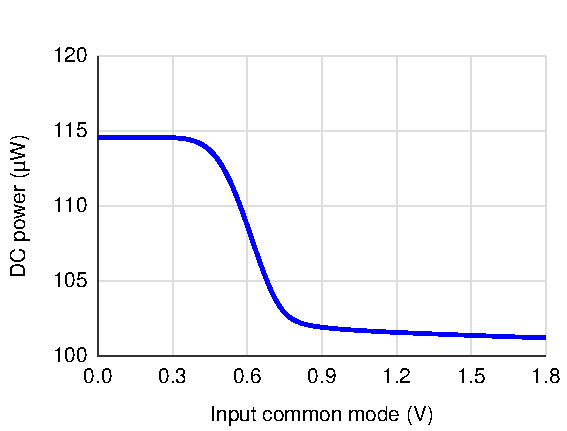
\includegraphics[width=\linewidth]{images/first-pass-power.pdf}
    \end{column}
  \end{columns}
\end{frame}

\begin{frame}{First-Pass Results --- Rejection, Slew Rate and Swing}
  \begin{columns}[T,onlytextwidth]
    \begin{column}{.586\textwidth}
    \begin{resulttable}
      \ade{CMRR_max_dB} & \(107.80\) dB & & \\
      \ade{PSRRp_max_dB} & \(99.47\) dB & & \\
      \ade{PSRRn_max_dB} & \(96.26\) dB & & \\[.45em]
      \ade{SR_RISING} & \(16.25\) V/\(\mu\)s & \(>20\) V/\(\mu\)s & \resultfail \\
      \ade{SR_FALLING} & \(16.85\) V/\(\mu\)s & \(>20\) V/\(\mu\)s & \resultfail \\[.45em]
      \ade{VDM_TRAN_at_5percent_THD} & \(2.34\,\mu\mathrm{V}\) & & \\
      \ade{OutSwing_Upper} & \(1.178\) V & & \\
      \ade{OutSwing_Lower} & \(0.623\) V & & \\
      \ade{OutSwing_Pk_Pk} & \(0.556\) V & & \\
    \end{resulttable}

    \medskip
    \footnotesize Output swing is measured at 5\% THD with a 100 Hz input.
    \end{column}
    \begin{column}{.382\textwidth}
      \centering\footnotesize Common-mode and supply rejection\par
      \smallskip
      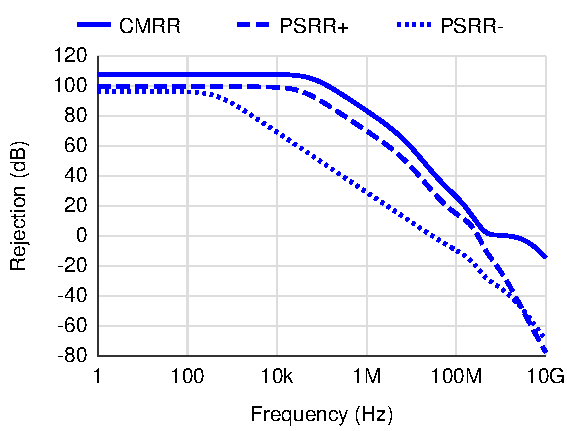
\includegraphics[width=\linewidth]{images/first-pass-rejection.pdf}
    \end{column}
  \end{columns}
\end{frame}

\begin{frame}{Sizing Changes for Slew Rate and Saturation}
  \small
  The first-pass rising and falling slew rates were 16.25 and
  16.85 V/\(\mu\)s. Both had to exceed 20 V/\(\mu\)s.
  At the DC operating point, M3 and M4 each supplied 9.90 \(\mu\)A.
  Each input transistor drew 8.21 \(\mu\)A, leaving only 1.69 \(\mu\)A
  for each folded branch (M5, M6) against a target of 5 \(\mu\)A.

  \medskip
  \footnotesize
  \renewcommand{\arraystretch}{1.15}
  \begin{tabular*}{\linewidth}{@{\extracolsep{\fill}}ll
      >{\raggedright\arraybackslash}p{.63\linewidth}@{}}
    \textbf{Device} & \textbf{\(W\) (\(\mu\)m)} & \textbf{Design change and outcome}\\
    \hline\noalign{\vskip .25em}
    M3, M4 & \(2\to4\) &
      More current in the folded branches raised falling slew to
      23.56 V/\(\mu\)s. M3 and M4 entered triode.\\[.5em]
    M5, M6 & \(2\to6\) &
      Widening the folded devices lowered the M3 and M4 drain voltages.
      Their final saturation margins were 82.5 and 81.5 mV.\\[.5em]
    M13 & \(6\to8\) &
      A wider output current source supplied more charging current.
      The final rising slew rate was 25.22 V/\(\mu\)s.\\
  \end{tabular*}
\end{frame}

\begin{frame}{Final Amplifier Core and Bias Network}
  \centering
  \makebox[\linewidth][c]{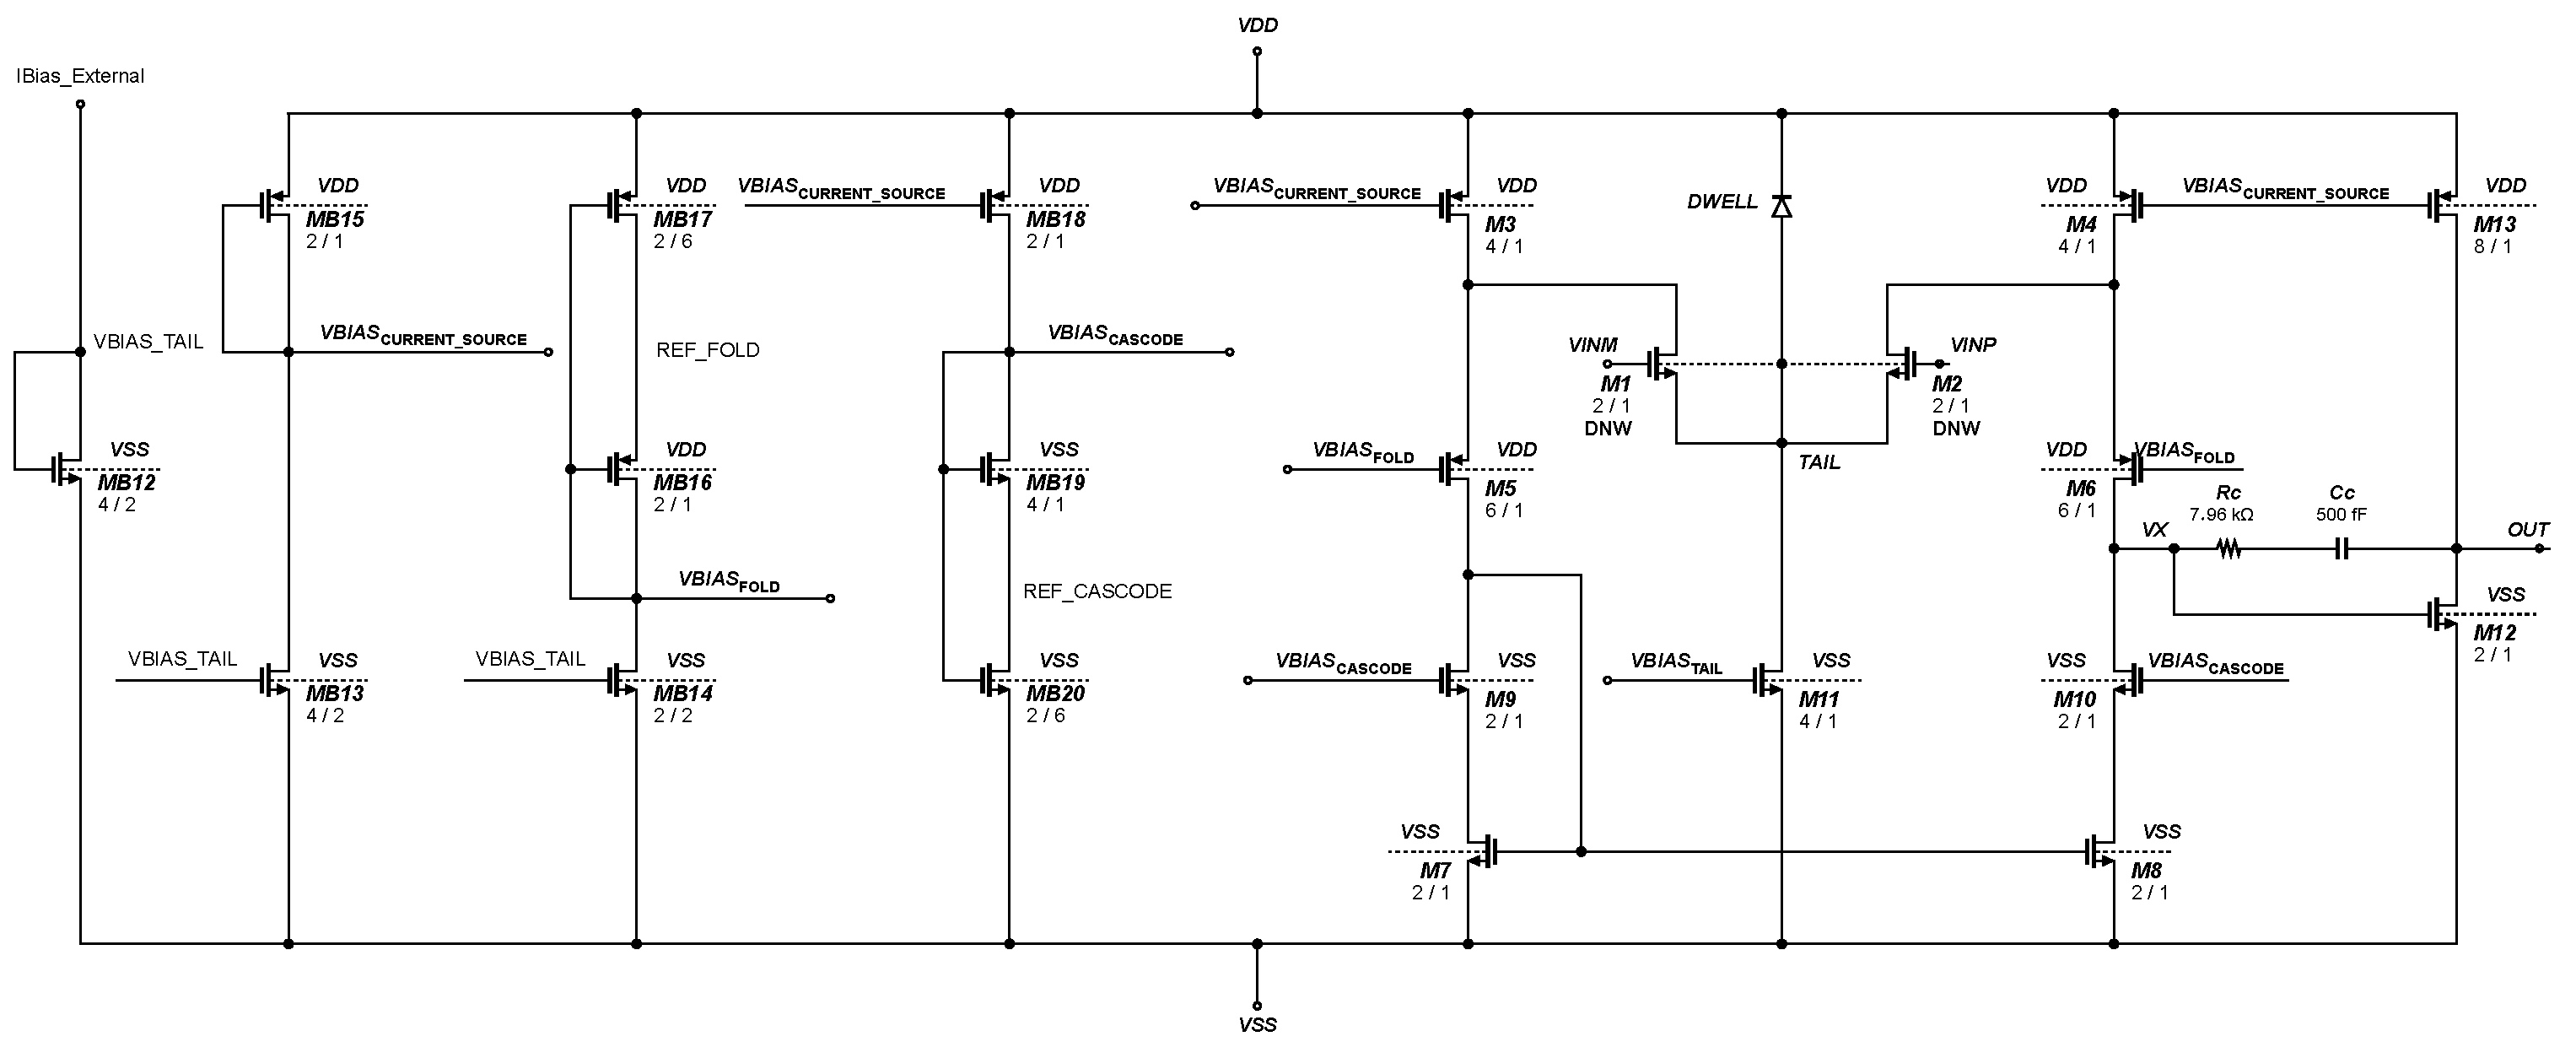
\includegraphics[width=.97\paperwidth]{images/final-core-and-bias.pdf}}
\end{frame}

\begin{frame}{Final Nominal Results --- DC and Differential Gain}
  \begin{columns}[T,onlytextwidth]
    \begin{column}{.586\textwidth}
    \begin{resulttable}
      \ade{Vout_CL} & \(0.900121\) V & & \\[.22em]
      \ade{VDM_OFFSET} & \(-105.71\,\mu\mathrm{V}\) & & \\[.22em]
      \ade{ICMR_Lower} & \(0.7545\) V & & \\
      \ade{ICMR_Upper} & \(1.79625\) V & & \\[.22em]
      \ade{PowerDC_nominal} & \(159.28\,\mu\mathrm{W}\) & & \\
      \ade{PowerDC_MAX_ICMR} & \(160.31\,\mu\mathrm{W}\) & \(<500\,\mu\mathrm{W}\) & \resultpass \\[.22em]
      \ade{A0_dB_1Hz} & \(102.80\) dB & \(>60\) dB & \resultpass \\
      \ade{fp1} & \(208.82\) Hz & & \\
      \ade{GBW} & \(28.91\) MHz & \(>20\) MHz & \resultpass \\
      \ade{UGF} & \(24.10\) MHz & & \\
      \ade{Phase Margin} & \(61.16^{\circ}\) & \(>45^{\circ}\) & \resultpass \\
    \end{resulttable}
    \end{column}
    \begin{column}{.382\textwidth}
      \centering\footnotesize\ade{PowerDC_vs_VCM}\par
      \smallskip
      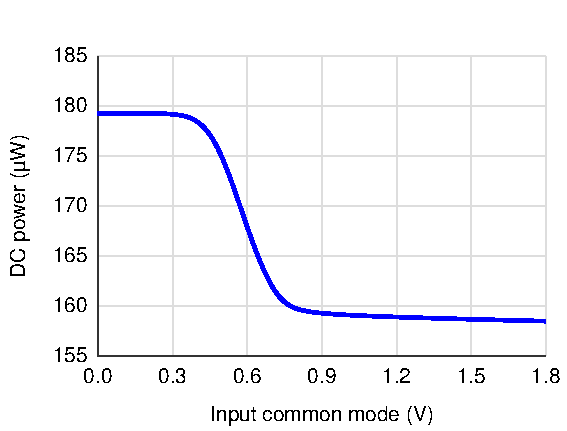
\includegraphics[width=\linewidth]{images/final-power.pdf}
    \end{column}
  \end{columns}
\end{frame}

\begin{frame}{Final Nominal Results --- Rejection, Slew Rate and Swing}
  \begin{columns}[T,onlytextwidth]
    \begin{column}{.586\textwidth}
    \begin{resulttable}
      \ade{CMRR_max_dB} & \(89.70\) dB & & \\
      \ade{PSRRp_max_dB} & \(85.02\) dB & & \\
      \ade{PSRRn_max_dB} & \(80.35\) dB & & \\[.45em]
      \ade{SR_RISING} & \(25.22\) V/\(\mu\)s & \(>20\) V/\(\mu\)s & \resultpass \\
      \ade{SR_FALLING} & \(30.49\) V/\(\mu\)s & \(>20\) V/\(\mu\)s & \resultpass \\[.45em]
      \ade{VDM_TRAN_at_5percent_THD} & \(4.32\,\mu\mathrm{V}\) & & \\
      \ade{OutSwing_Upper} & \(1.245\) V & & \\
      \ade{OutSwing_Lower} & \(0.567\) V & & \\
      \ade{OutSwing_Pk_Pk} & \(0.679\) V & & \\
    \end{resulttable}

    \medskip
    \footnotesize Output swing is measured at 5\% THD with a 100 Hz input.
    \end{column}
    \begin{column}{.382\textwidth}
      \centering\footnotesize Common-mode and supply rejection\par
      \smallskip
      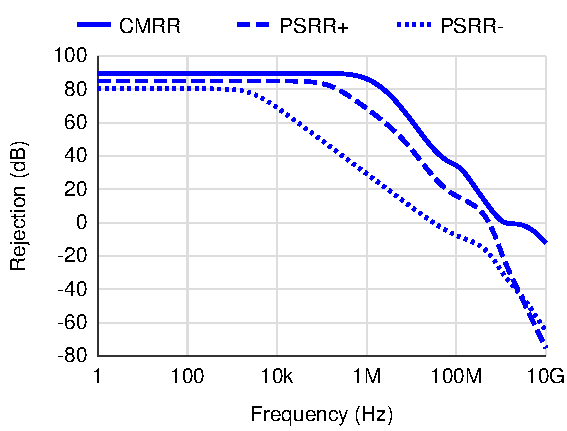
\includegraphics[width=\linewidth]{images/final-rejection.pdf}
    \end{column}
  \end{columns}
\end{frame}

\endgroup
\end{document}
